\chapter{Implementation}
\label{Ch5}
%\setcounter{page}{1}
%\pagenumbering{arabic}
\bigskip

The setup we have is like this:
Computer Name: Dell\\
Computer OS: Ubuntu 16.04 LTS\\
Runtime Platform:\\
	Server: Localhost, Apache, MySQL, PHP, PHP-MyAdmin\\
	Client: Browser (Chrome, FireFox), JavaScript-5, Active Internet Connection\\

The list of tools and important functions used:
\begin{itemize}
\item Image API
\item File API
\item SHA-256
\item Base-64
\item Image
\item AES
\item RSA
\end{itemize}
	


We have tried to make basic blockchain platform without video processing right now for a single node processing. The screenshot of the process is the following,


\begin{figure}
\begin{center}
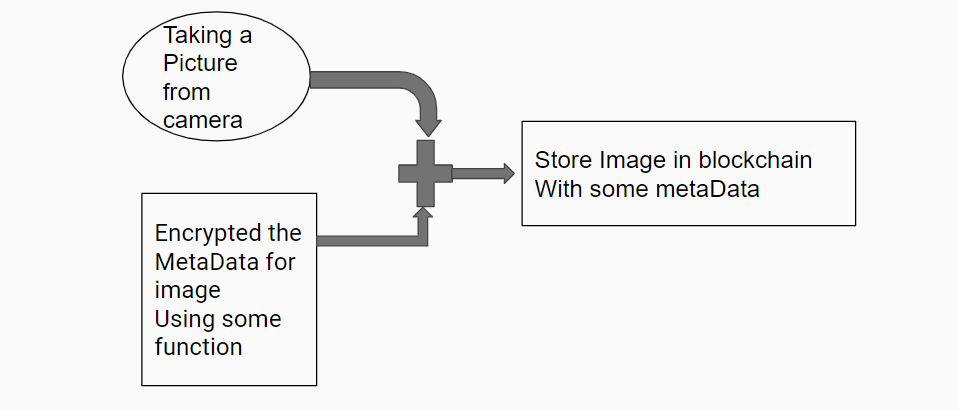
\includegraphics[width=0.75\textwidth]{./img_src/upload.png}
\end{center}
\caption{Image Insertion}
\end{figure}

\begin{figure}
\begin{center}
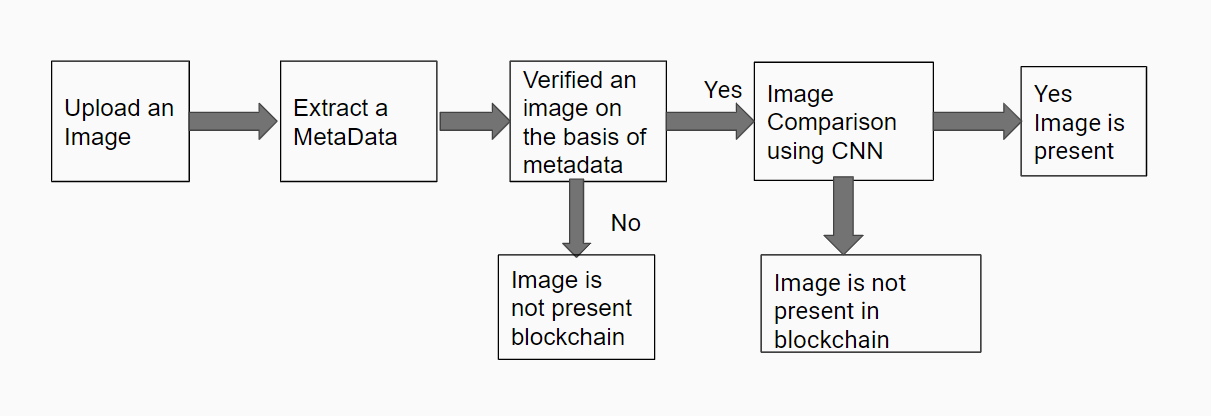
\includegraphics[width=0.75\textwidth]{./img_src/verify.png}
\end{center}
\caption{Image Verification}
\end{figure}


\begin{figure}
\begin{center}
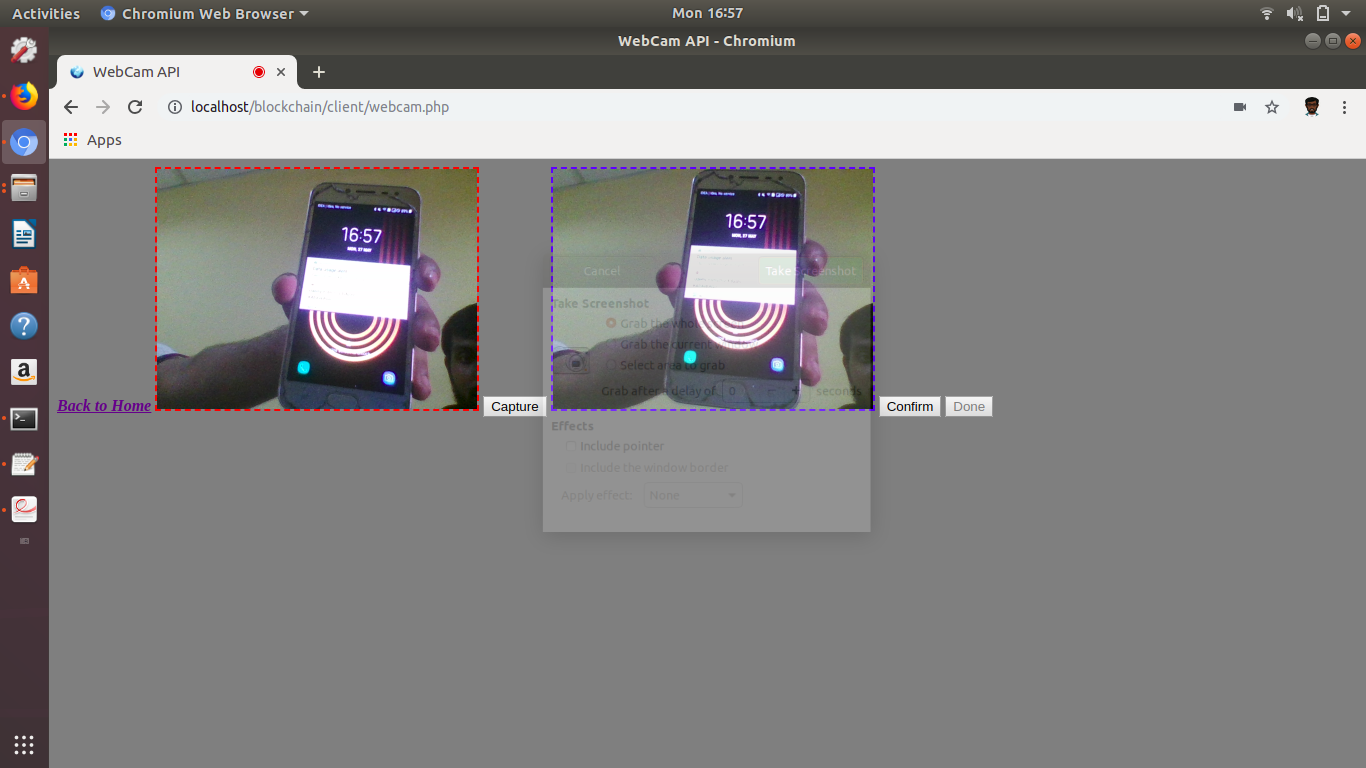
\includegraphics[width=0.75\textwidth]{./img_src/screen1.png}
\end{center}
\caption{Image Verification}
\end{figure}


\begin{figure}[!htb]
%\center{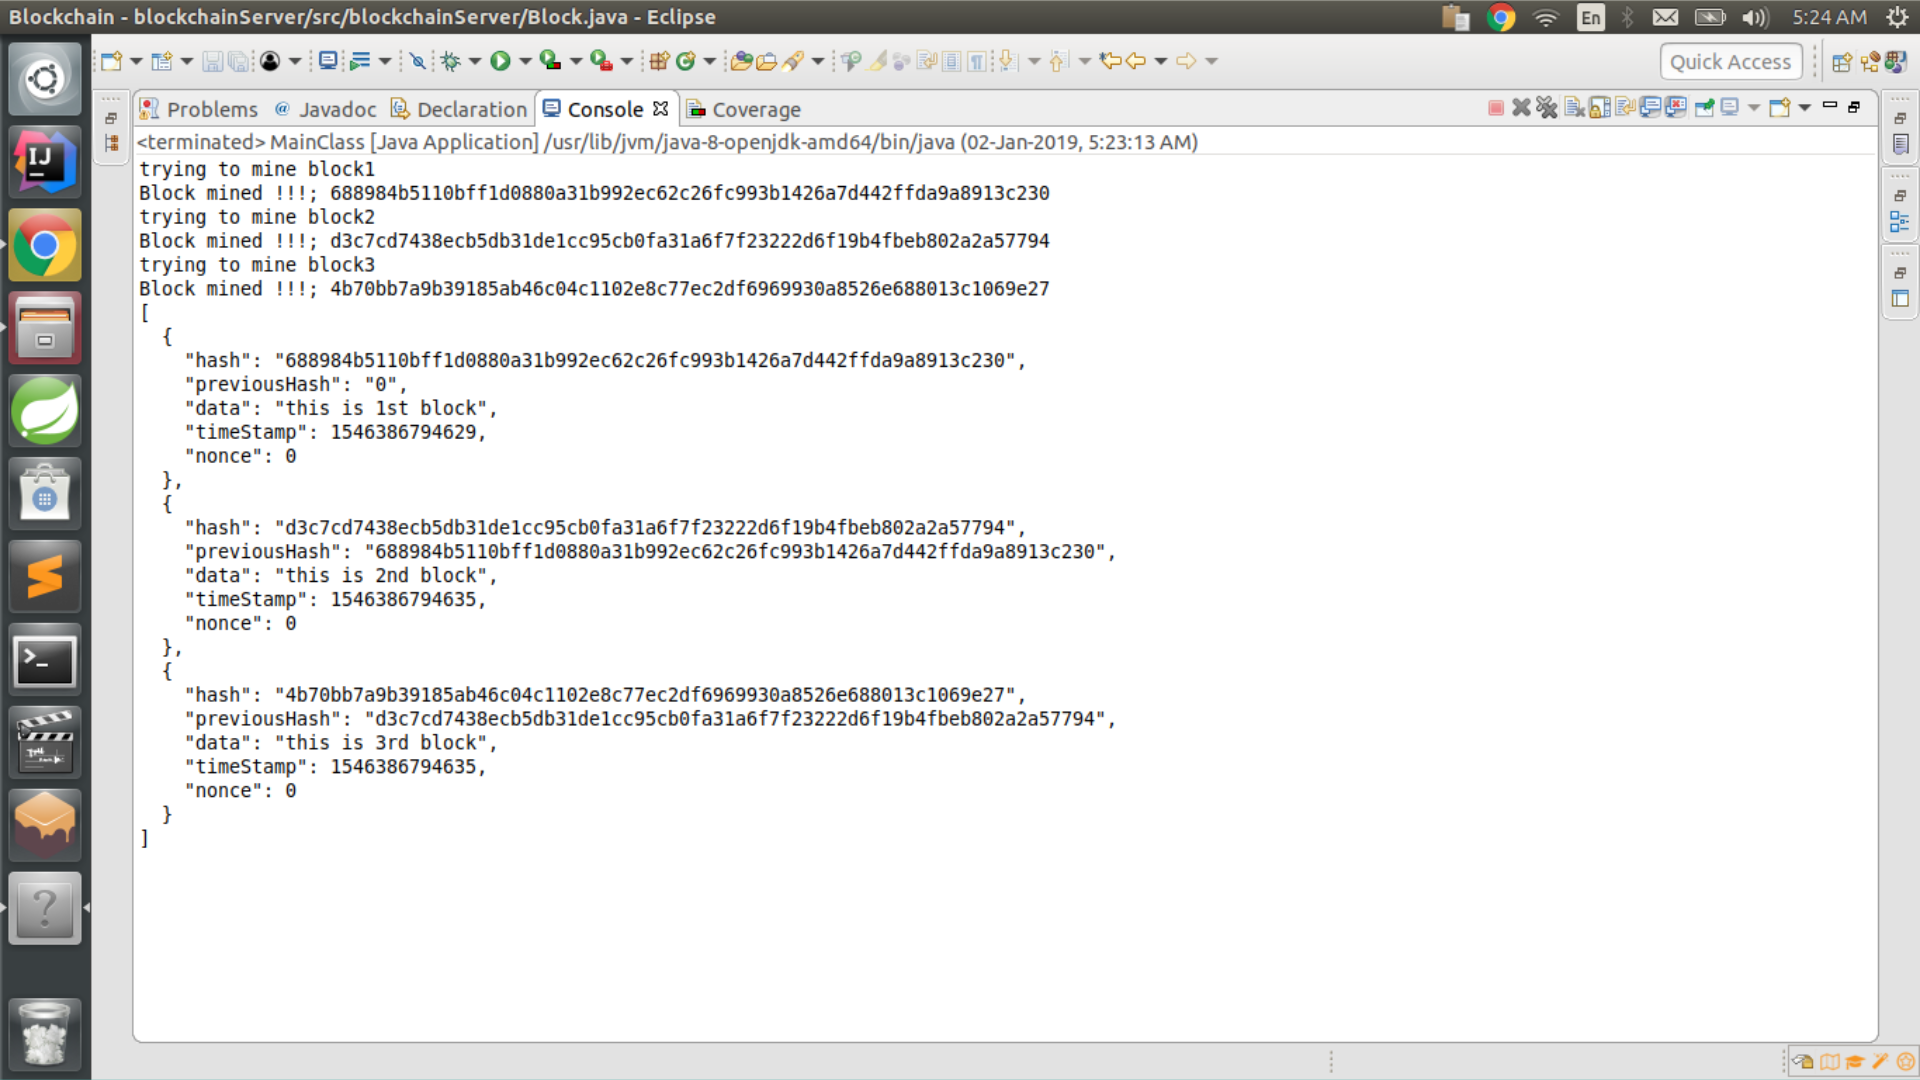
\includegraphics[width=\textwidth]{p0.png}}
\caption{\label{fig:my-label}. Implementation Runtime in Terminal}
\end{figure}

This picture shows how we have created the basic blockchain platform with the following tools:
\begin{itemize}
\item Image API
\item SHA-256
\end{itemize}
There is a very simple concensus mechanism we have used to create the temporary (as the blocks are created and destroyed in the logical memory by Computer Program) private (as right now it is residing in our computer, not in a web server) ledger.\\

As we are implementing in Java, there are publicly functioning classes along with a class containing main function.\\
The classes we have are:\\
	Block\\
	Transaction\\
	String Utility\\
	Main\\

The String Utility contains some manipulation with the SHA-256 program, implemented by Java.\\

The Block contains the following:
Id, 
Timestamp, 
Data, 
Prev hash, 
Nonce\\

For containing the hashes we are using List datatype in Java. Before adding any block we are checking 3 things, that are:\\
Timestamp: The time that it has been created\\
Previous Hash: parent for current block\\
Nonce: Consensus mechanism\\

while using CreateBlock() and MineBlock()

In the transaction class we have,
	Source Name (Hash): transaction from\\
	Destination Name (Hash): transaction to\\

From main, we are
	creating transactions: calling Transaction class
	visiting transactions: receiving hashes


We have planned to include online platform the following way,

\begin{figure}[!htb]
%\center{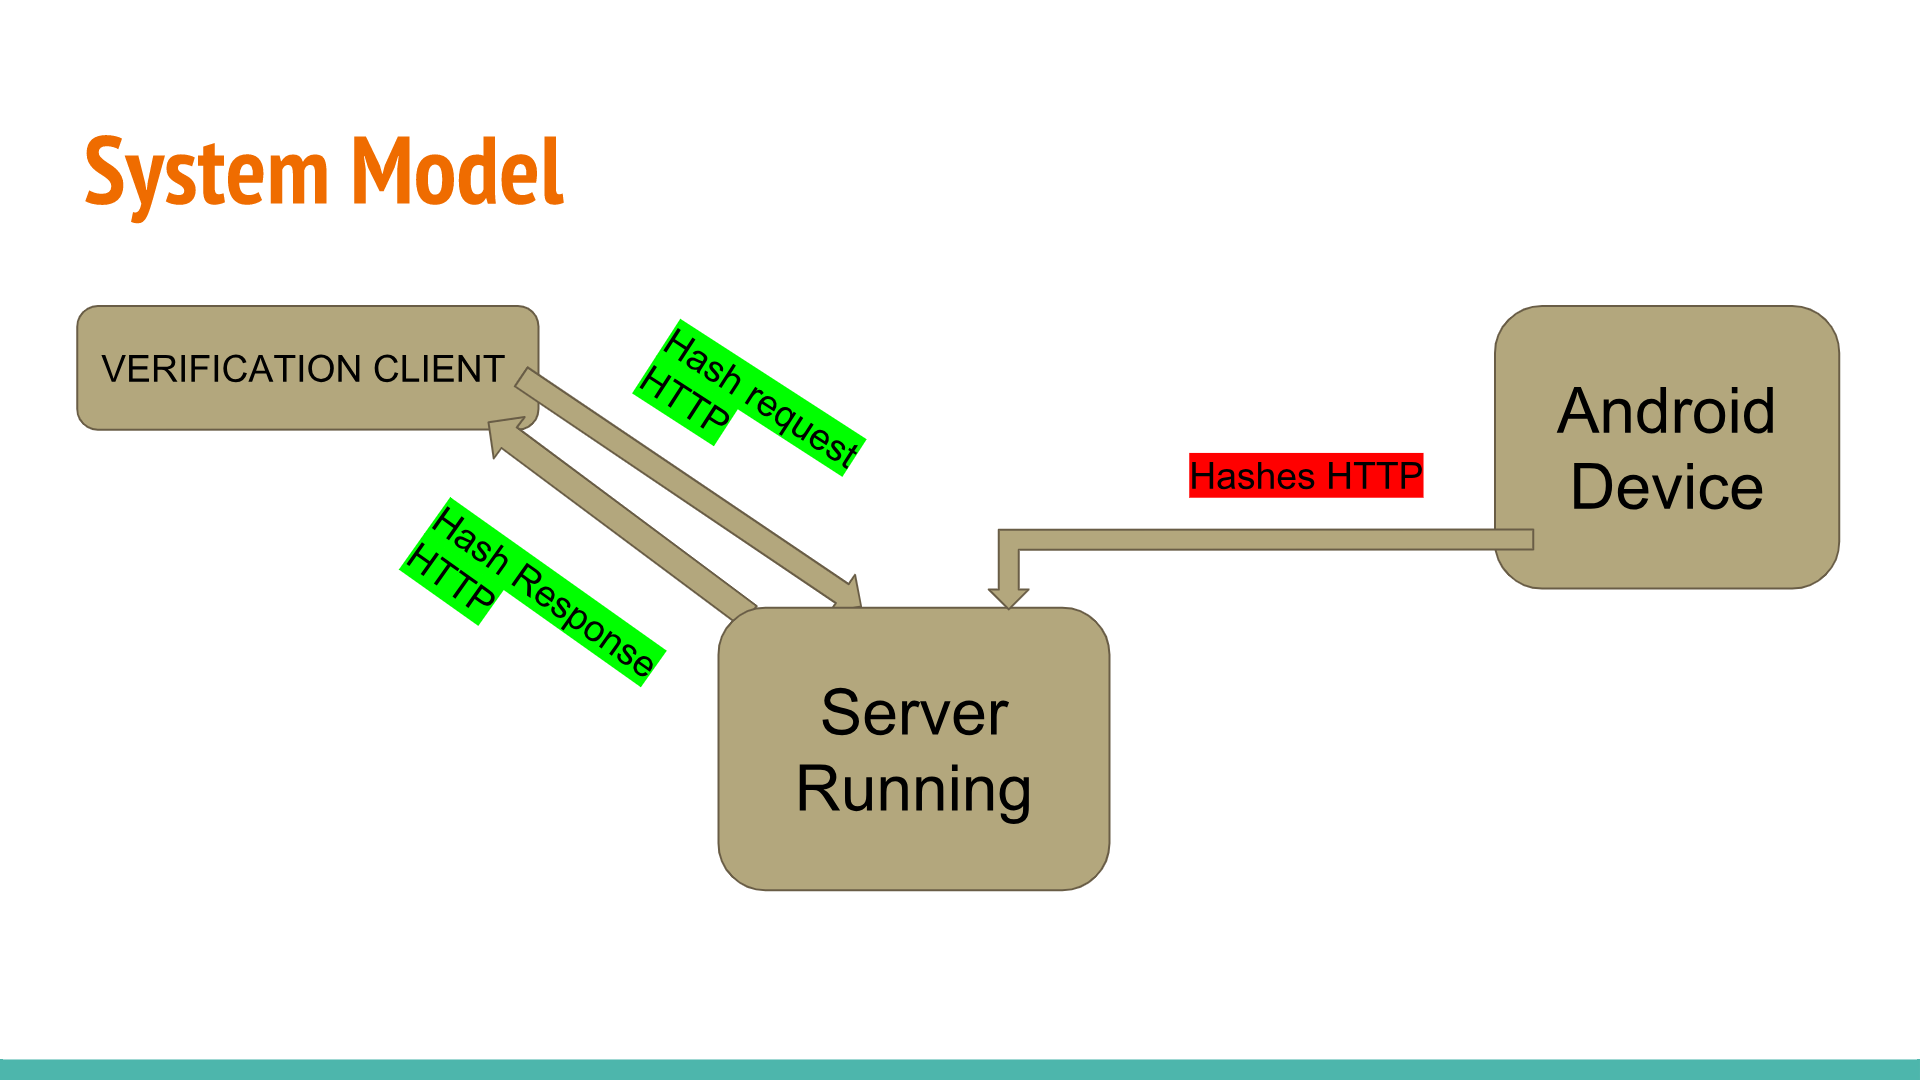
\includegraphics[width=\textwidth]{p1.png}}
\caption{\label{fig:my-label}. System Model}
\end{figure}

In this model we are suggesting that there should be client-server system before involving into the blockchain system. So user have to login first with the hashed id and password. Then the person can apply for either Storing data into system or verify data from the system. The Server will perform the task.\\

\begin{figure}[!htb]
%\center{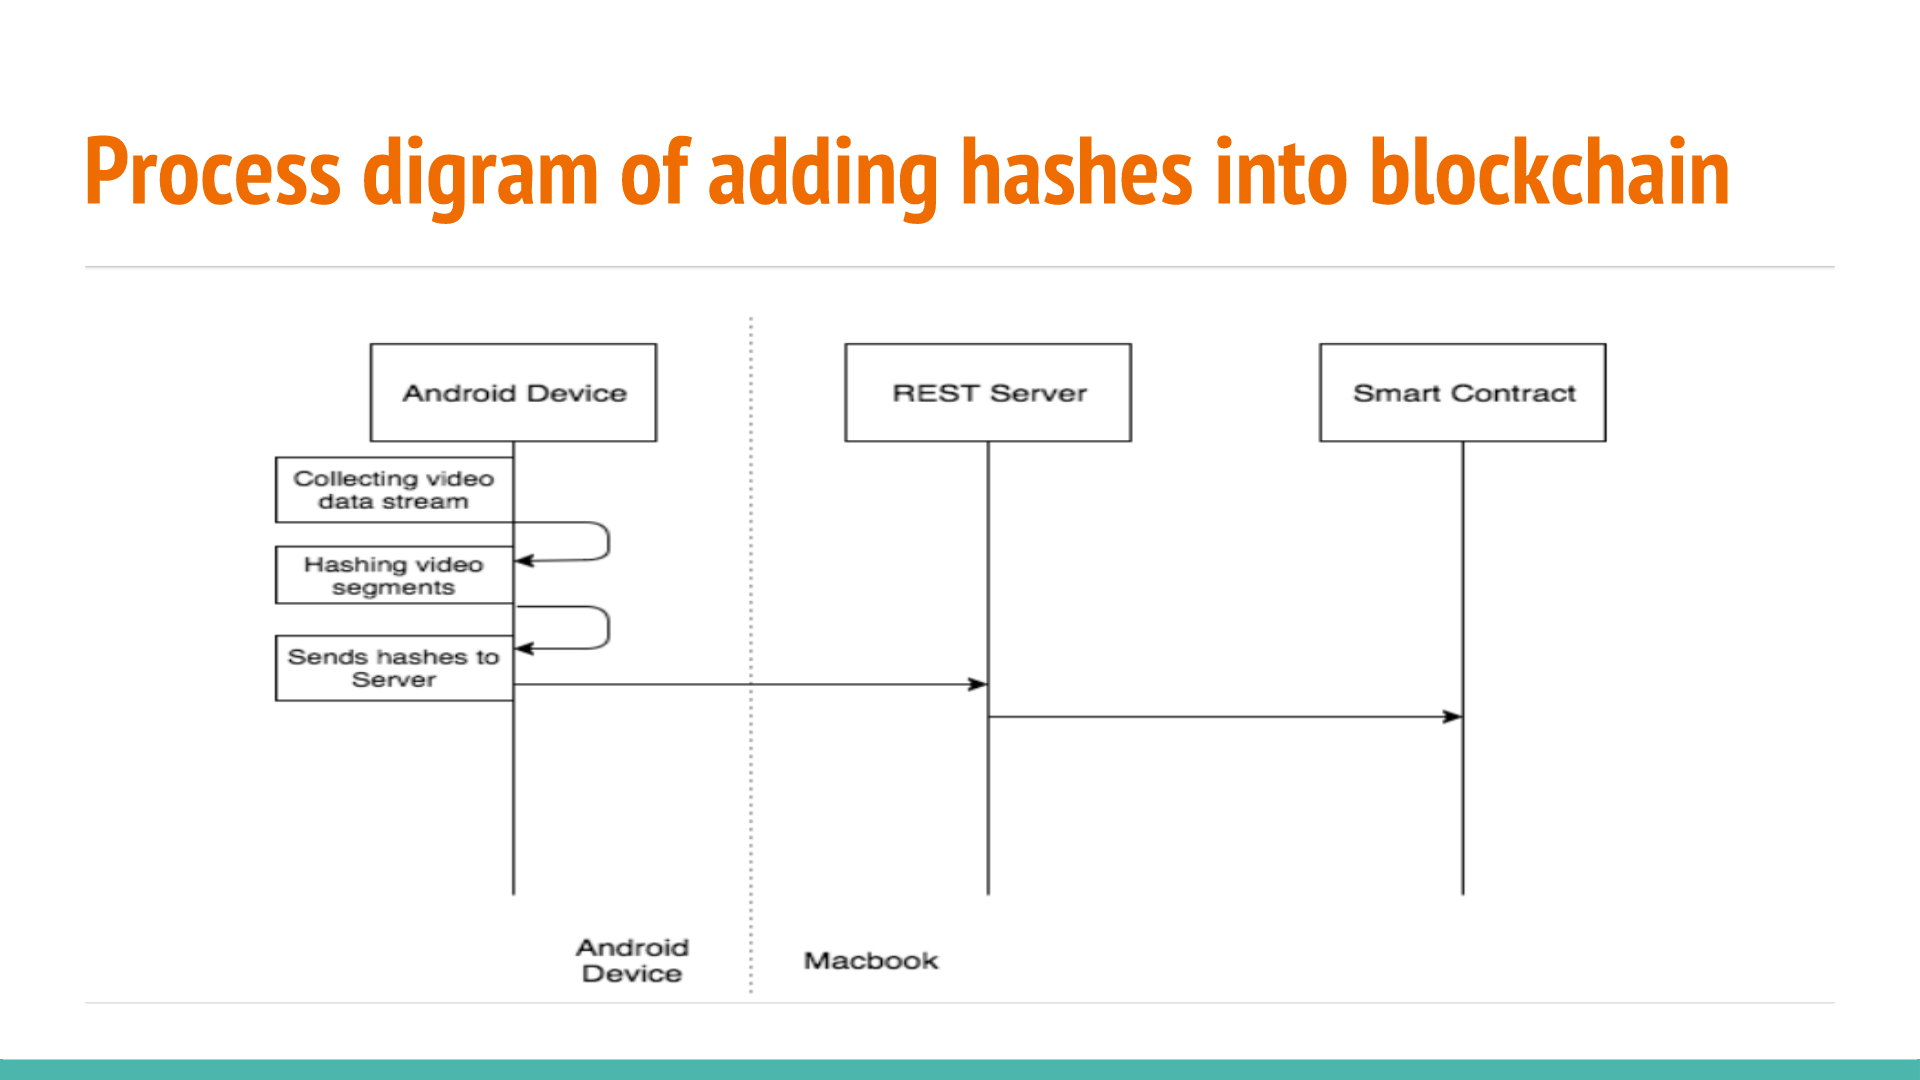
\includegraphics[width=\textwidth]{p2.png}}
\caption{\label{fig:my-label}. Process Diagram with Hashes}
\end{figure}

\begin{figure}[!htb]
%\center{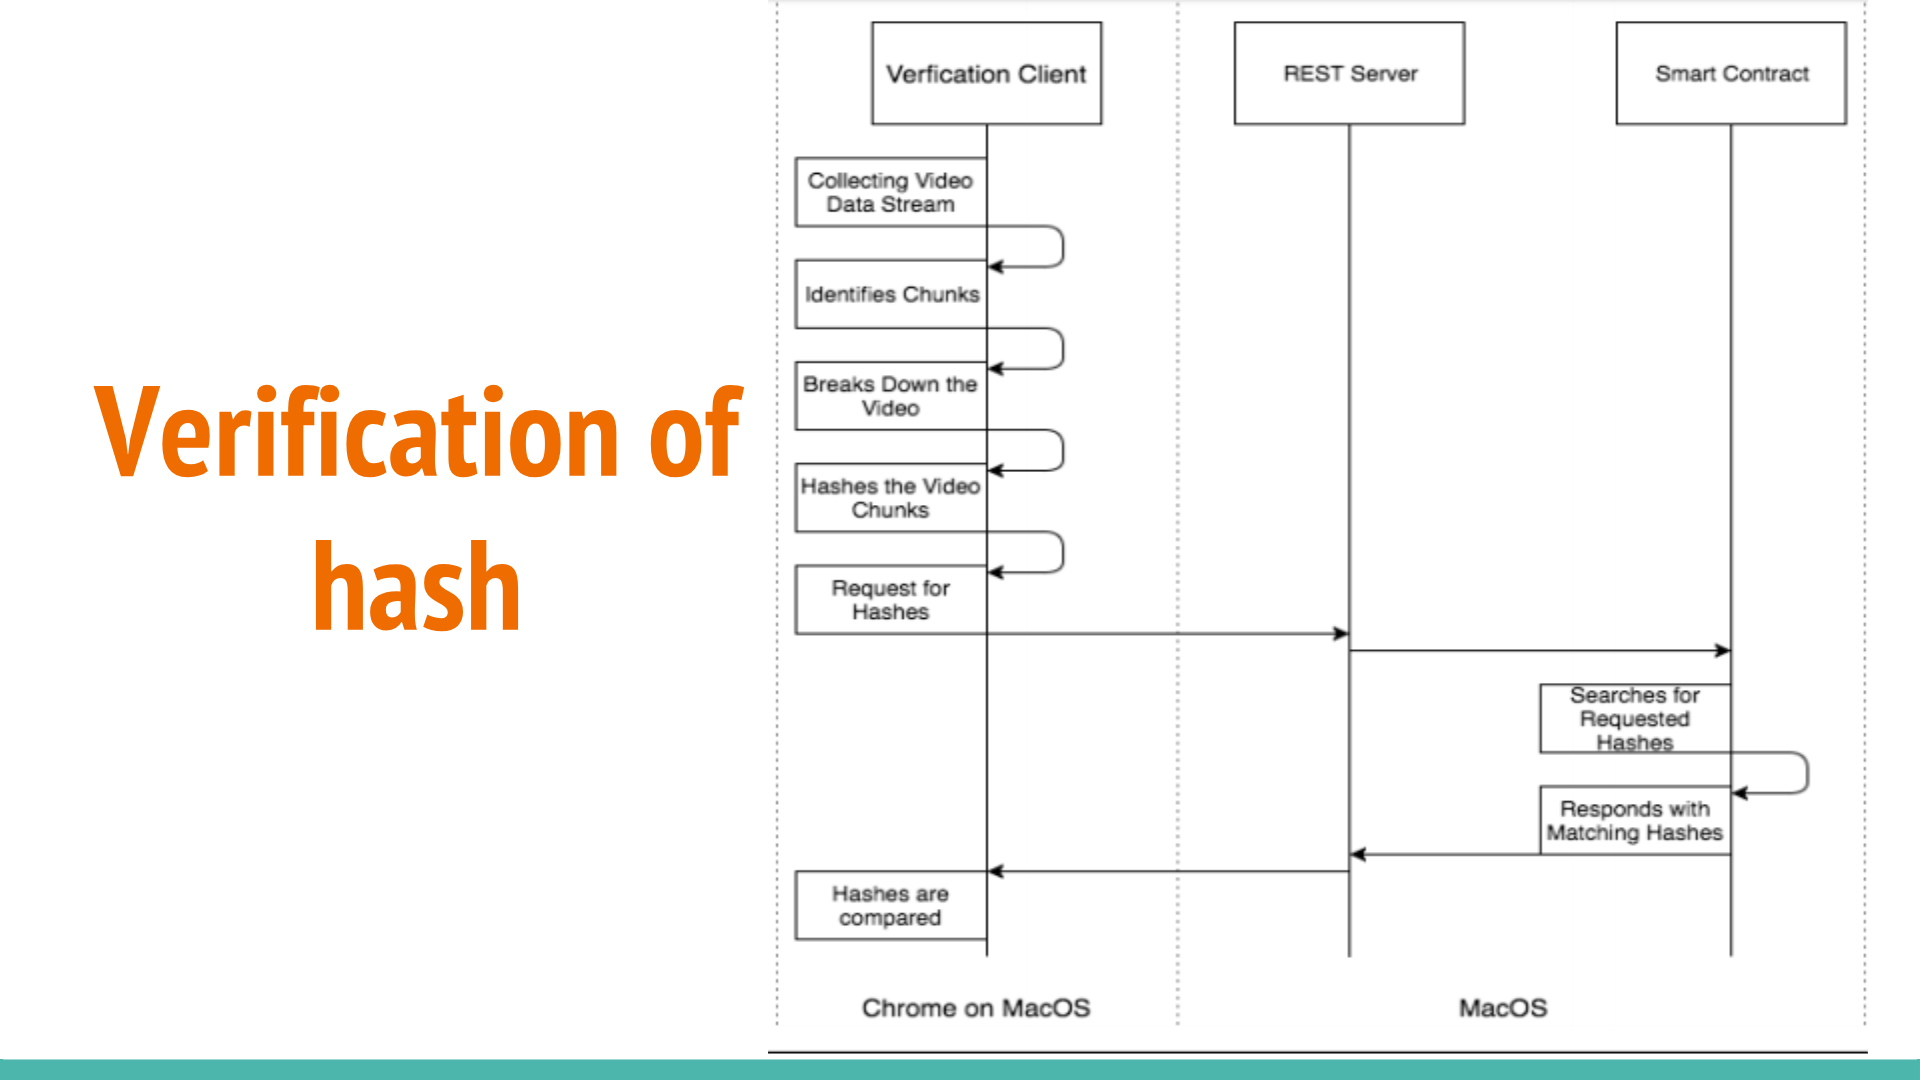
\includegraphics[width=\textwidth]{p3.png}}
\caption{\label{fig:my-label}. Verification Hash}
\end{figure}

